%!TEX root = ../template.tex
%%%%%%%%%%%%%%%%%%%%%%%%%%%%%%%%%%%%%%%%%%%%%%%%%%%%%%%%%%%%%%%%%%%%
%% chapter4.tex
%% NOVA thesis document file
%%
%% Chapter with lots of dummy text
%%%%%%%%%%%%%%%%%%%%%%%%%%%%%%%%%%%%%%%%%%%%%%%%%%%%%%%%%%%%%%%%%%%%
\chapter{Implementation of the \textit{iCBD-Replication and Cache Server}}
\label{cha:impl_replication_caching}

%This chapter addresses the implementation of the central topics of this thesis, divided into two major fields.
%We first start with a section talking about the creation of a middleware system that provides replication features in an integrated way to the iCBD platform. While providing a detailed description of the concept and architectural model, as well as the implementation decisions, made along the accomplishment of this contribution.
%Next, we show the work done on improving the performance of the platform clients. Displaying how setting up a client-side caching system that stores images adjacent to the consumers obtain that sought enhancements. Concluding in exploring the challenges of recreating the complete platform in a new environment and implementing a real-world scenario at Nova University Computer Science department laboratories. This chapter is partitioned as follows :

%will at last state the problem and motivation for introduction replication techniques in the storage components of the platform. Moreover, the section prefaces the importance of the implementation of cache servers that hold part of the distribution burden and crucial for the support of an increased number of clients. 

This chapter is about the core of this thesis: the iCBD-Replication and Cache Server, a middleware
system that provides replication features in an integrated way to the iCBD platform. Naturally, the first subsection provides a detailed description of the motivation, architecture and design aspects while the second subsection concentrates on the implementation. Finally, the last subsection deals with the process of building the Replication and Cache Server: that is, how the modules are installed and deployed in an iCBD infrastructure.

% TODO Cap4 - Rever estes pontos
\begin{description}
	\item [Section~\ref{sec:impl_mot_sysarch}] begins by explaining the motivation for the implementation of a replication module within the iCBD platform, as well as explaining the need to include a new role in the platform with the creation and deployment of a cache server near the clients. Concluding with the overall architecture of the system and how both topics complement each other.
    %
    \item [Section~\ref{sec:impl_icbdrep}] overviews the implementation of the middleware dubbed iCBD-Replication. Beginning the journey through the initial architectural process and then showing the implemented components and their interaction with the several layers of the platform.
    %
    \item [Section~\ref{sec:impl_cache_server}] shows how the complete iCBD platform was installed in the NOVA University cluster. Then, a description of the work performed to include a client-side caching server directly connected to the final clients.
    %
\end{description}
\newpage

%%-------------------------------------------------------------------
%%	4 - Motivation and System Architecture
%%-------------------------------------------------------------------
\section{Motivation and System Architecture}
\label{sec:impl_mot_sysarch}

One of the key objectives of iCBD is to provide a platform that can stretch from a fully hosted, on-site architecture to one where an important part of its services is cloud-based. Naturally, in-the-middle solutions are also interesting, such as one where, e.g., both the administration and storage of \textit{“golden”} iMIs are cloud-based, while the rest is on-premises. Therefore, it becomes evident that data locality is an important subject, and thus one must study how data flows between the components of the iCBD platform – a complex, data-intensive platform, boasting multiple storage devices and many different networks, accessed by multiple consumers demanding data at any given time.

All these factors, allied to the desire of having a distributed and scalable platform architecture, result in the need to design a new service whose mission is to ensure that data is correctly replicated in the appropriate places, and consistency of the various versions of the iCBD Machine Images stored is maintained. This led to the high-level architecture of Figure~\ref{fig:impl_icbd_rep_arch_simple}

%\subsection{Motivation}
%\label{sub:impl_mot}

%\subsection{System Architecture}
%\label{sub:impl_sysarch}

\begin{figure}[htbp]
    \centering
    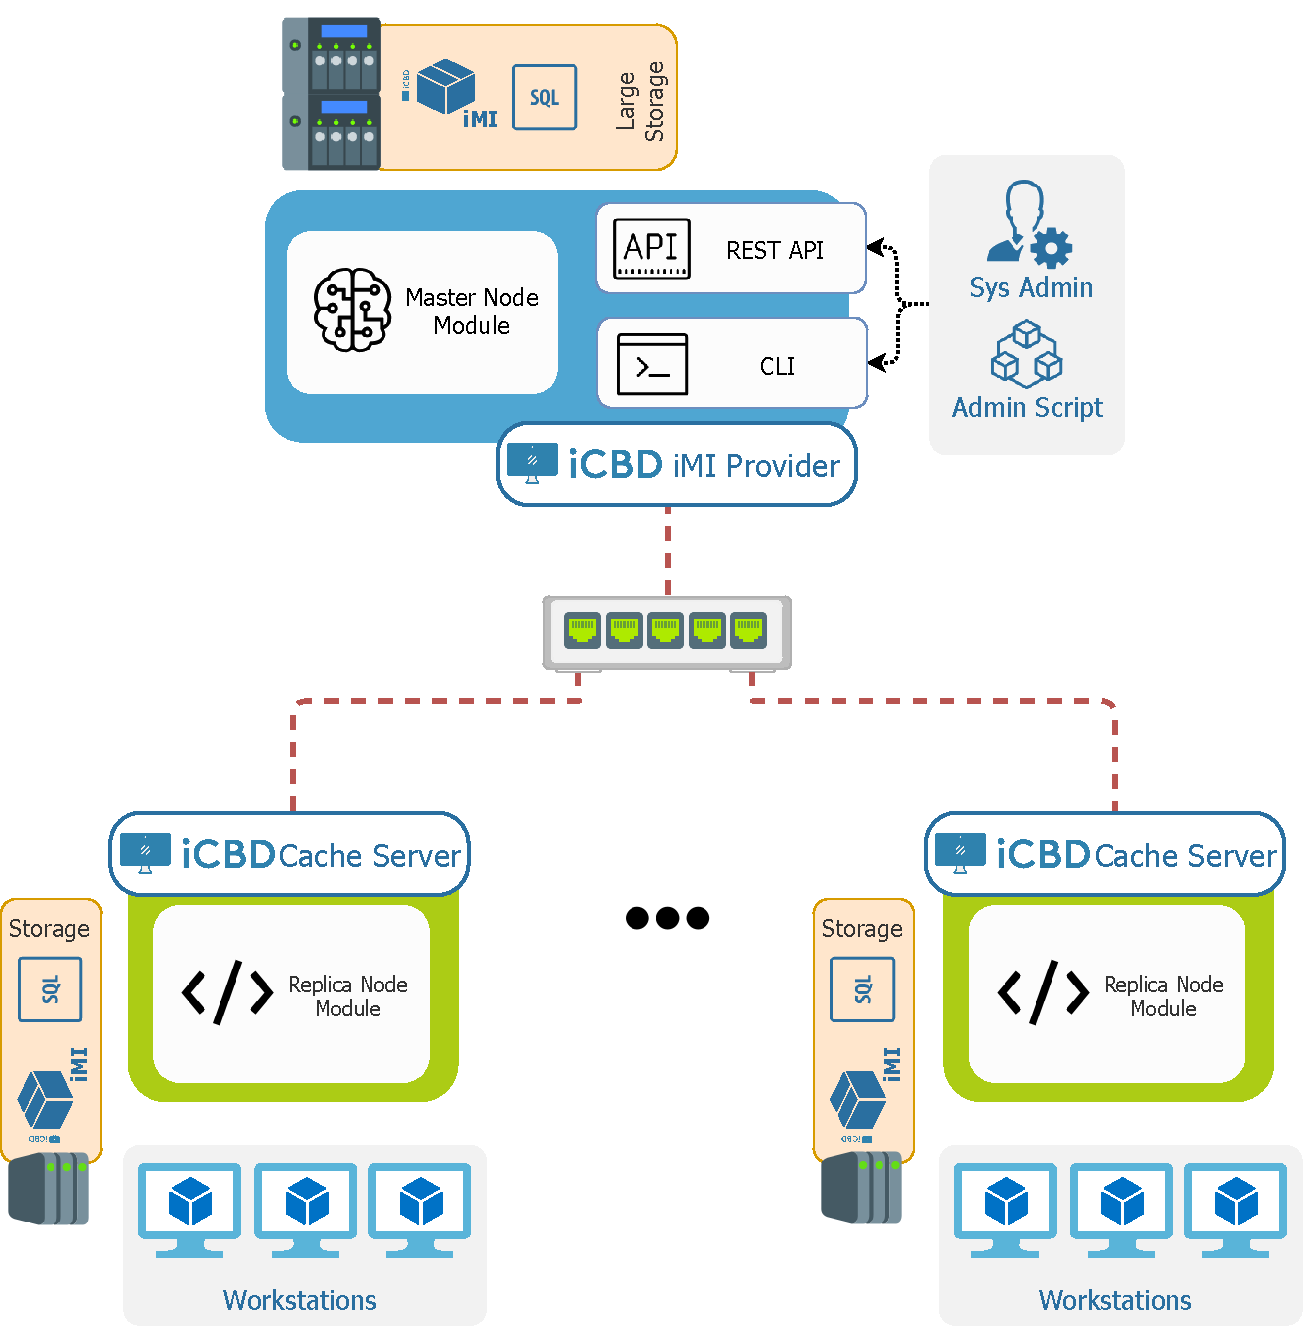
\includegraphics[height=4in]{cap4_icbd_rep_simple}
    \caption{iCBD Replication and Caching Architecture (high-level)}
    \label{fig:impl_icbd_rep_arch_simple}
\end{figure}

%%-------------------------------------------------------------------
%%	4 - Implementation of a Replication Module
%%-------------------------------------------------------------------
\section{Implementation of a Replication Module}
\label{sec:impl_icbdrep}

%One of the central objectives of iCBD is to provide a platform that can be both cloud-centric, with the administration and a portion of the storage burden gathered in a public cloud, or fully hosted on client premises. Either way, it becomes evident that data locality is an important subject, which means that there is the necessity to study how this data will flow between the multiple components of the iCBD platform.
%As can be imagined, this is a data-intensive platform, boasting multiple storage devices in many networks and an array of consumers demanding that data at any given time.

%All these factors allied to the platform architecture result in the need to create a new component, whose chief mission is to ensure that the data is correctly replicated in the appropriate places, maintaining the consistency of the various versions of the iCBD Machine Images stored.

When our project started, iCBD was already available; therefore, our Replication and Caching Service (from now on, RCS) had to be integrated with the existing architecture and support (and enhance) the previous work. This influences the choices available for the RCS implementation and could, in a worst-case scenario, severely limit them. Fortunately, that was not the case.

iCBD was designed from the start based on the assumption that the storage layer where iMIs live was built on top of a storage system which supports snapshots. In the first prototype, Btrfs was chosen for the storage layer but, in theory, any storage system that supports snapshots can be used in the platform. That is, in fact, the case with a parallel work being developed in another dissertation, where the focus is the use of an object-based storage system, Ceph.


%%-------------------------------------------------------------------
%%	4. - Requirements of the Module
%%-------------------------------------------------------------------
\subsection{Requirements}
\label{sub:impl_requirements_icbdrep}

%\textbf{TOPICS :}
%The file system is set BTRFS will be used.
%Many reasons for that:
%The most important is the support for snapshots
%Compression

%Since the beginning of this work, the file system selected for use in the storage layer was selected, this is due to the fact that, there was already a functioning prototype of the core iCBD platform making use of BTRFS for all data storage matters. The most critical feature for the operation of the platform is that the file system supports snapshots. BTRFS is a modern file system based on the copy-on-write (COW) principle capable of creating lightweight copies of a file. We detailed the importance of this trait in Section~\ref{sub:icbd_storage_layer}.
 
%The condition described above applies only in the choice of the File System, in theory, any File System that supports snapshots can be employed in the platform. That is, in fact, the case with the work developed in a dissertation carried out in parallel to this one, where the focus is the use of an object-oriented file system, in particular, the CEPH File System.
%Due to this imposition, it is key that this work makes the best use of the BTRFS features, exploring the incremental backup capabilities. More, the replication process should fully integrate with the core platform that already distributes iMIs to clients. Preservation of consistency of the iMIs is also a concern, assuring the distribution of new versions when they are created.

%Moreover, it should be taken in account the locality of the data, since the communications could originate and end in the same data centre and the same local network, or happening between different locations that can be in opposite sides of the world. Such aspects as the bandwidth used and the encryption of the data becomes essential to address, requiring the examination of several compression algorithms that can be accommodated to the way the data is processed and also ways of keeping this data secure by encrypting the communications.

Btrfs is a modern file system based on the concept of copy-on-write (COW): it is capable of creating lightweight copies of filesystem structures – files, directories, volumes. We already detailed the importance of this trait in Section~\ref{sub:icbd_storage_layer}. Therefore, a mandatory step was to investigate Btrfs-provided tools that could help us to achieve our primary goal: being able to move information (“base” iMIs and their snapshots) around, from “master” to “secondary” nodes, while consuming the minimum bandwidth – one must not forget that, while a typical Linux iMI is less than 10 GB, a Windows 10 iMI is circa 40 GB. We found that Btrfs has incremental backup capabilities, and therefore we set out to explore those.
 
So,  Btrfs’s incremental backup capabilities are a good starting point; however, their purpose is to help in data transfer; but that is not enough. Preservation of consistency of the iMIs is also a concern, as one has to assure that iMIs cached in the RCSs are up-to-date, and when a new iMI is created its distribution will start “immediately”, to ensure high availability in case of faults. Moreover, the locality of the data should be taken into account, since data transfer endpoints may be located within the same data centre, or at, e.g., geographically disperse regions in the world. Bandwidth use and data encryption become essential, requiring the study of compression algorithms and encryption techniques.


%\subsubsection{Preliminary tests on the BTRFS Incremental Backup features}
\paragraph{BTRFS Incremental Backup feature}
\label{par:impl_incremental_btrfs}

%A first step is trying to understand the most efficient way to transfer this unique kind of data (i.e. an iMI). Given the fact that we are working with a file system with snapshots capabilities, we want to take advantage of this functionality and minimise the amount of data roaming the network.

%The BTRFS developers provide a userspace set of utilities that can manage BTRFS filesystems, called \texttt{btrfs-progs}. Within that set of tools, there is a pair of commands, \texttt{btrfs send}~\cite{btrfs_send}, and \texttt{btrfs receive}~\cite{btrfs_receive}, that provides the capability to transport data via a stream and employ those differences in a remote filesystem. 

%The send command facilitates the process of generating a stream of instructions that describe changes between two subvolume snapshots. Also available in the command is the ability to use an incremental mode, where given a parent snapshot that is available in both send and receive sides, only the small delta between snapshots (e.x. \textit{V2} and \textit{V2-1} in fig~\ref{fig:icbd_rep_imi_snap}) is going to integrate the stream. This feature is outstanding since considerably reduces the amount of information that needs to be transferred to reconstruct the snapshot in the receiving end. The send side operations occur in-kernel, beginning by determining differences within subvolumes and based on those differences the kernel generates a set of instructions in a custom formulated stream.

%On the remote end, the received command accepts the stream generated by the send command and uses that data to recreate one or more snapshots. Contrary to the send command, receive executes in user space, replaying the instructions that come in the stream one by one, these instructions include the most relevant calls found in a Virtual File System, with Unix system calls like \texttt{create()}, \texttt{mkdir()}, \texttt{link()}, \texttt{symlink()}, \texttt{rename()}, \texttt{unlink()}, \texttt{write()}, along with others.~\cite{btrfs_design}

A first step is trying to understand the most efficient way to transfer this unique kind of data (i.e. an iMI). Given the fact that we are working with a file system with snapshots capabilities, we want to take advantage of this functionality and minimise the amount of data roaming the network.

Btrfs has a set of userspace utilities to manage Btrfs filesystems, called \texttt{btrfs-progs}; these include a pair of commands, \texttt{btrfs send}~\cite{btrfs_send}, and \texttt{btrfs receive}~\cite{btrfs_receive}, that provide the capability to transport data via a stream and apply differences from/to a remote filesystem. The send command simplifies the process of generating a stream of instructions that describe changes between two subvolume snapshots. Also available is the ability to use an incremental mode, where given a parent snapshot that is available in both the send and receive sides, only the small delta between snapshots (e.x. V2 and V2-1 in Figure~\ref{fig:icbd_rep_imi_snap}) is going to integrate the stream. This feature considerably reduces the amount of information that needs to be transferred to reconstruct a snapshot in the receiving end. The send-side operations occur in-kernel, beginning by determining differences within subvolumes and, based on those differences, the kernel generates a set of instructions in a custom-formulated stream.

\begin{figure}[htbp]
    \centering
    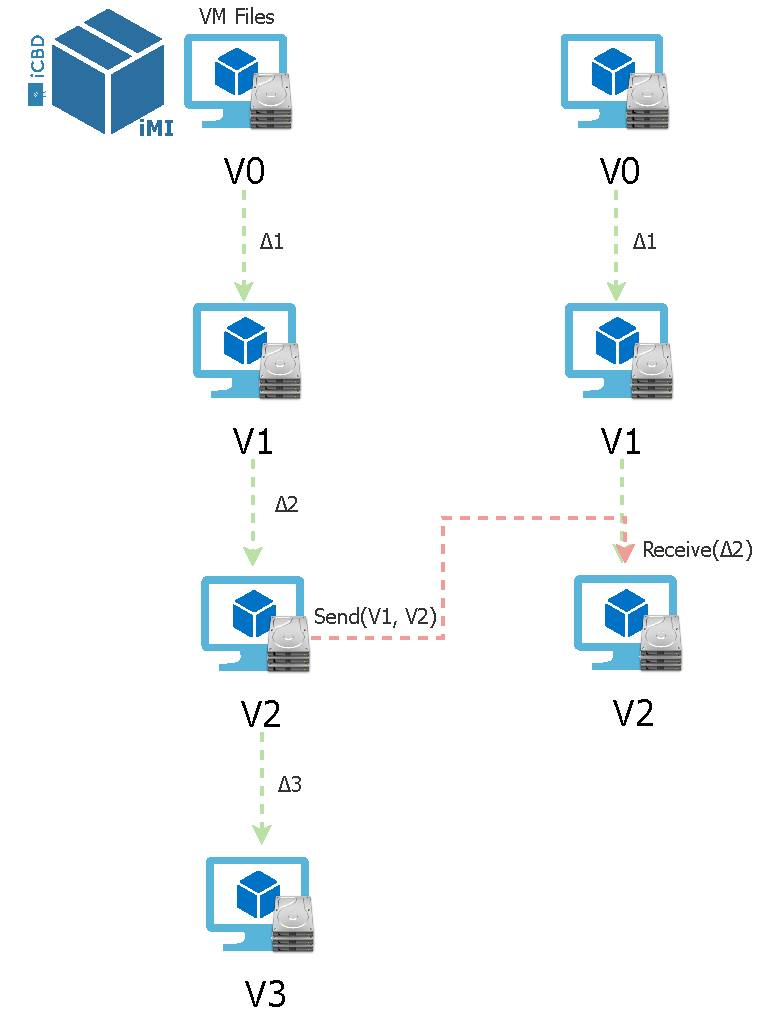
\includegraphics[height=4in]{cap4_iMI_deltas}
    \caption{iCBD iMI Snapshots Structure}
    \label{fig:icbd_rep_imi_snap}
\end{figure}

On the remote end, the receiving command accepts the stream generated by the send and uses that data to recreate one or more snapshots. Contrary to the send command, receive executes in user space, replaying the instructions in the stream one by one; the set of instructions includes the most relevant calls found in a Virtual File System, such as \texttt{create()}, \texttt{mkdir()}, \texttt{link()}, \texttt{symlink()}, \texttt{rename()}, \texttt{unlink()}, and \texttt{write()}, along with others~\cite{btrfs_design}.


%https://btrfs.wiki.kernel.org/index.php/Incremental_Backup
%https://www.samba.org/ftp/rsync/rsync.html



%%-------------------------------------------------------------------
%%	4. - System Overview
%%-------------------------------------------------------------------
\subsection{System Overview}
\label{sub:impl_system_overview}


\begin{figure}[htbp]
	\centering
%	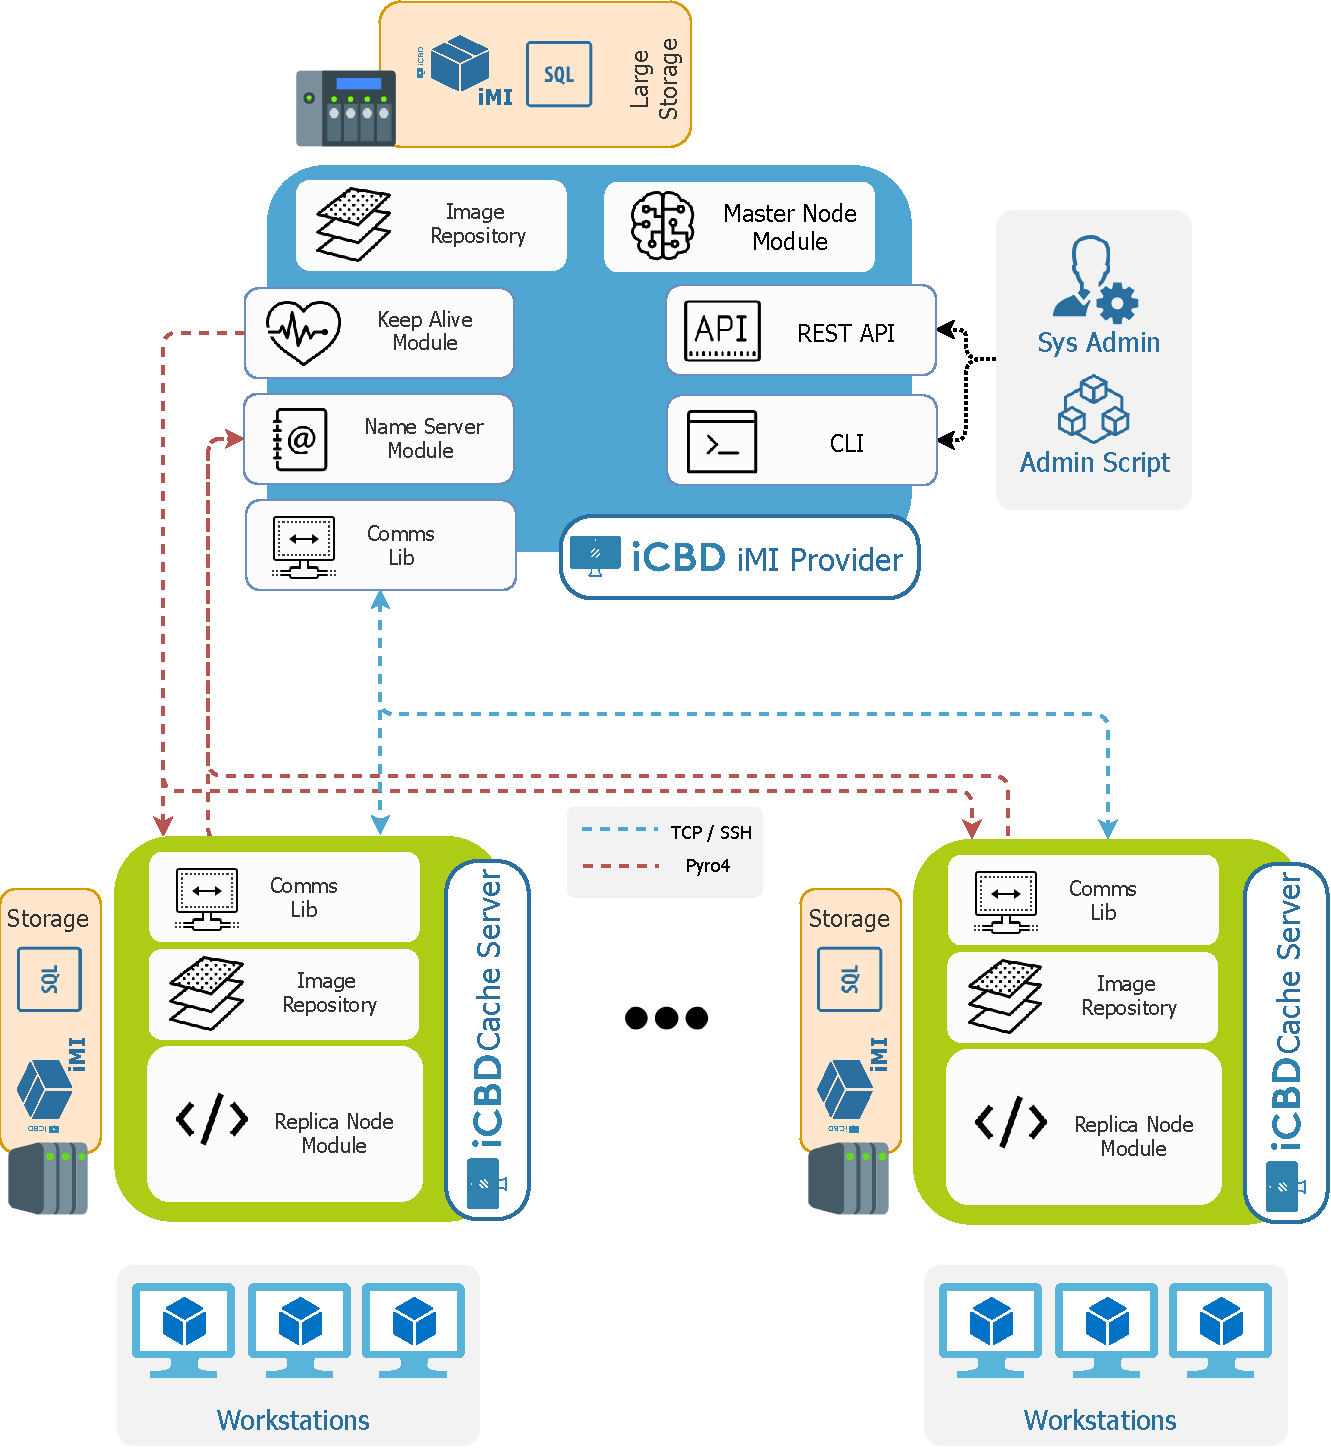
\includegraphics[height=4in, width=\textwidth]{cap4_icbd_arquit}
	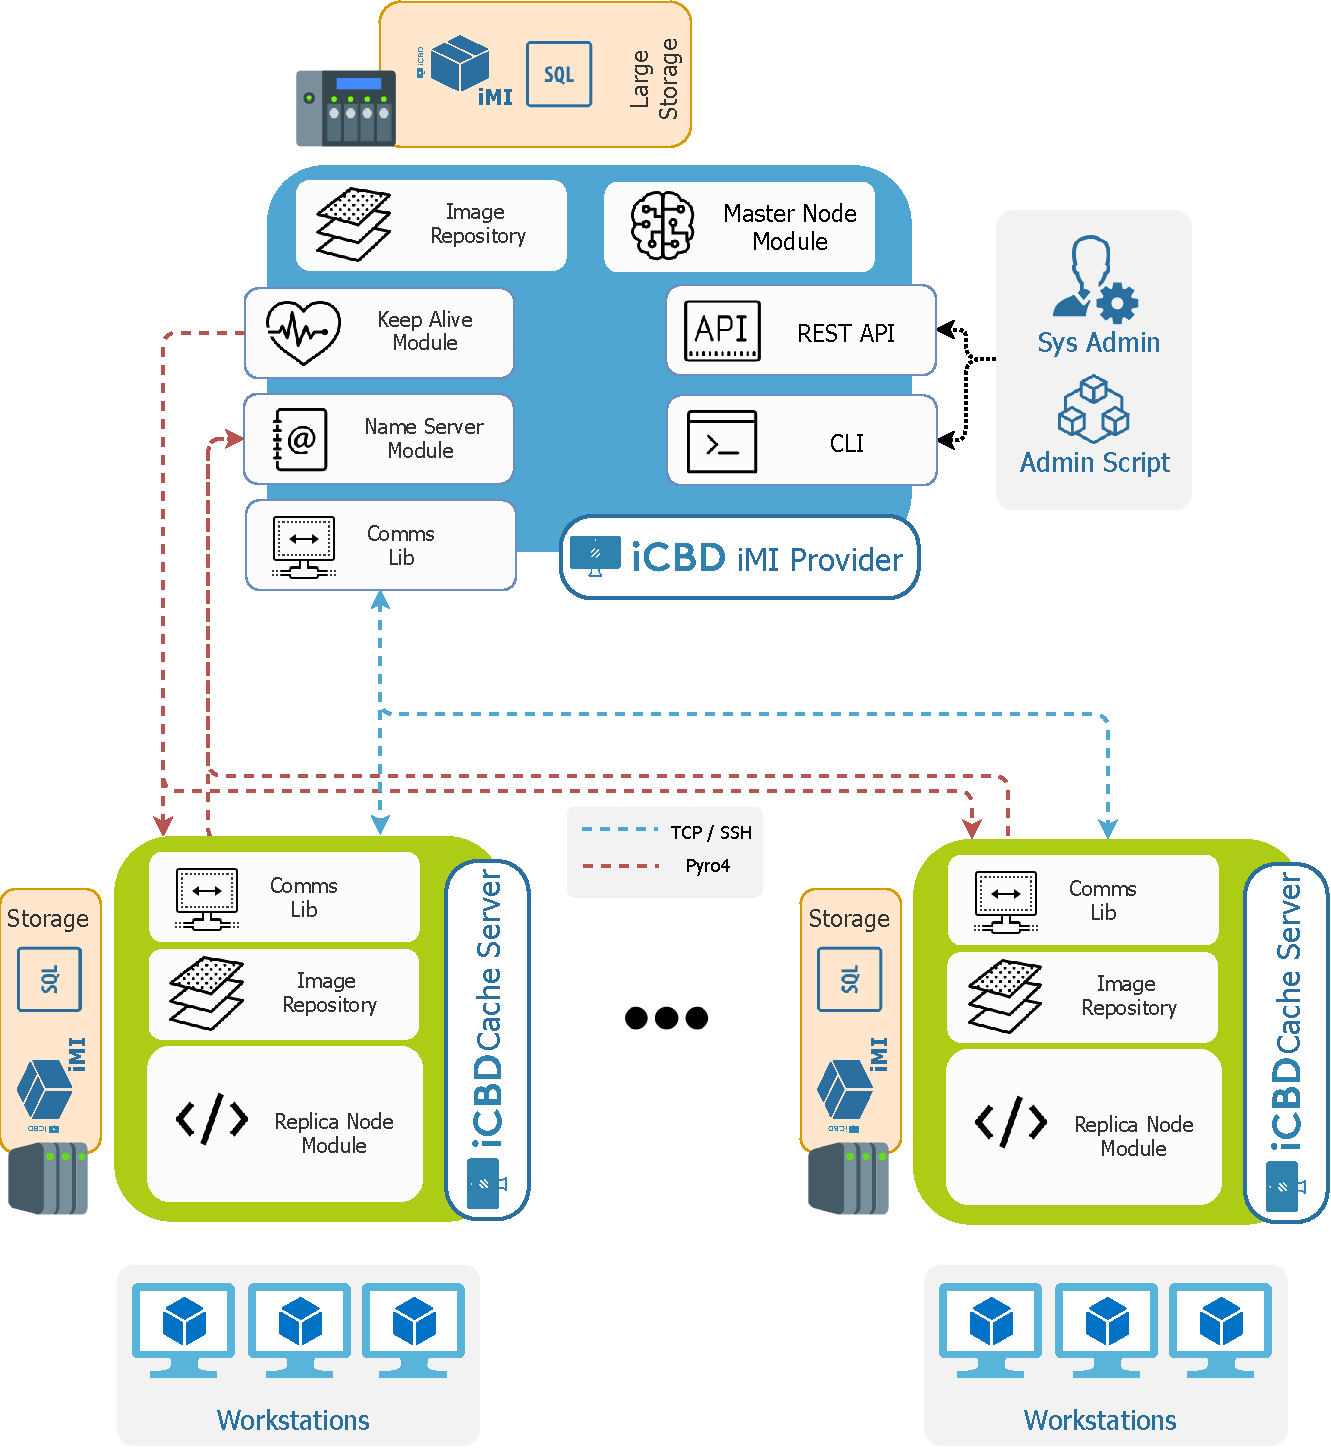
\includegraphics[width=\textwidth]{cap4_icbd_arquit}
	\caption{iCBD Replication Modules and Communications}
	\label{fig:icbd_rep_mods_comms}
\end{figure}
 
%Since the replication module needs to interact with several bash scripts, with the core iCBD platform, including command line tools and some operating systems low-level features, we betted that the most suitable approach was creating a python distributed middleware using a master-replica paradigm.

%Python as a programming language enjoys some valid idiosyncrasies, functioning as an object-oriented language, possessing an extensive standard library and enjoys a big community delivering packages with a wide range of functionality, all facts that contribute to make it the best programming language to bundle everything together.

%The several modules of the middleware comprise the main functionalities allowing a node to behave as a Master or Replica node, where each one maintains its individual Image Repository. Then there are also a number of libraries that were developed to interface with some tools, as the BTRFS tool talked about above~\ref{par:incremental_btrfs}, to interface with an SSH connection, build wrappers for compression algorithms and even provide a REST API.

%An overview with a small description of the functionality of each component of the system follows:

Since the replication module interacts with different tools and utilities, e.g., bash scripts and command line tools and some OS calls, we think that the most suitable approach was to create a Python distributed middleware layer using a master-replica paradigm.

Python, as a programming language, enjoys some idiosyncrasies, functioning as an object-oriented language, possessing an extensive standard library and enjoying a big community delivering packages with a wide range of functionality; all these facts contribute to make it the most appropriate programming language to bind everything together in our iCBD platform.

Our middleware is composed of several modules and includes all the necessary functionalities that allow a node to behave as a Master or as a Replica, where each maintains its individual Image Repository. A number of libraries were also developed: to interface with some tools, such as Btrfs send / receive and with SSH, to build wrappers for compression algorithms, and even to provide a REST API.

An overview with a small description of the functionality of each component of the RCS system follows:

\begin{description}
	\item [Master Node] This node acts both as a controller to the replication system and an interface to interact with a client whether through a CLI or REST API. This node shall reside on an iCBD Administration machine since it must deliver changes made to iMIs to all replicas. It is also responsible for communicating with the Name Server to gather information about which nodes are present on the platform, or what is their status; even instruct the replicate nodes to execute certain operations.
	%
	\item [Replica Node] Its main task is to maintain the list of subscribed iMIs that are not up-to-date, receive the updates as soon as the Master Node sends them, and store them locally. Upon request, the Replica Node can deliver the list of iMIs that are locally stored and their version numbers, and subscribe (or unsubscribe) for new IMIs.
	%
	\item [Name Server] This service lives in the same machine as the Master Node, holds records about nodes in the replication system, in a phone book type simple database. Nodes register themselves in the name server during the startup process (and leave on shutdown) and can, at any moment, query about the location of other nodes.
	%
	\item [Keep Alive] It's a Master Node thread that periodically checks if Replica Nodes are still operating correctly. When it identifies that a replica node is no longer responding, it immediately sends a request to the for the removal of the dead node from the Name Server’s directory.
	%
	\item [Image Repository] This module is a custom-made data structure that holds a (large) set of iCBD Snapshot objects in a \texttt{key:value} store. In addition to storing these objects, it has an interface that provides quick answers to queries that ask which iMIs are stored in the node’s repository. Every node in the platform (i.e. Master or Replica) must necessarily hold one repository.
\end{description}


%So that all the components presented above can function adequately, they require help from several libraries. A description of those implemented libraries ensue:

All the previously described components interact with a number of “objects”, so it is not a surprise that a sizeable amount of code that we have created has been packed into a number of libraries:

\begin{description}
	\item [BTRFS Lib] The Btrfs library holds two classes: the first one, called \texttt{Btrfs Tool}, is a Python wrapper for \texttt{btrfs-progs}, described in section~\ref{par:impl_incremental_btrfs}.; the other class, designated \texttt{BtrfsFsCheck} implements functions that validate if a given path transverses a Btrfs filesystem and, if it does, verifies if in that path a subvolume also exists. Additionally, a method is provided to discover all snapshots in a directory.
	%
	\item [Compression Lib] Since multiple compression algorithms are used, it makes sense to create a library that encapsulates multiple wrappers, one for each algorithm; these wrappers only contain code that provides compression and decompression of data streams, no other operations are present.
	%
	\item [Serialiser Lib] Some communication operations between nodes require the transmission of objects; therefore a library containing serialisation and deserialisation methods for those objects has been implemented.
	%
	\item [SSH Lib] This library implements a wrapper for the SSH command, allowing the creation of tunnels so that data can be funnelled through a secure connection between nodes.
	%
	\item [REST API Lib] To comply with one of the objectives of the replication module, a REST API should be provided. That is precisely what this library does, providing the endpoints to interact with the system, and enabling an easy way to expand that interaction to other platform modules.
\end{description}

%Even though the libraries presented above are not enough for the appropriate implementation of the all functionalities of the replication module, more libraries implemented by the community were necessary to handle aspects like communication between nodes, algorithms for data compression and to secure the data transmission between networks. Some of which we list and describe below  (a full list of Python packets imported in the project is shown in the Listing~\ref{listing:impl_icbd_pipfile}), also throughout the remaining text we detail in each module the libraries that help to accomplish its purpose.

The libraries we created to implemented the common set of functionalities required for the replication module, do require more libraries, implemented by the Python community. These are necessary to handle communication between nodes, algorithms for data compression, and secure data transmission; the most relevant ones are described through the remaining text in this section.

\begin{listing}[ht]
\inputminted{python}{./Chapters/Code/cap4_pip.py}
\caption{Dependences of the iCBD-Replication module bundled in a Pipfile}
\label{listing:impl_icbd_pipfile}
\end{listing}


%%-------------------------------------------------------------------
%%	4. - Communications between nodes
%%-------------------------------------------------------------------
\subsection{Communications between nodes}
\label{sub:impl_rep_comms}

%Coordinate the multiple modules and its activities, demands from the middleware a need to share a communication channel connected through a network. 
%The remote procedure call (RPC) brings support for inter-process communication allowing a procedure on a system to invoke an operation running in a process in a different location, most likely on a remote system.

%As seen in figure~\ref{fig:icbd_rep_mods_comms}, multiple processes are running in different machines any given time, and those processes need to continually send and receive information: perhaps operations to execute, metadata updates, or just monitoring if a process is running according to the desired plan or is in a faulty state.
%Managing the nodes is a perfect case for the use of the Pyro 4 library, that gives a holistic view of the system and allows triggering a multitude of operations in each node.

To coordinate the multiple modules and their activities, an abstraction of a network-shared communication channel must be supported. The remote procedure call (RPC) was chosen to support the inter-process communication, allowing a procedure running on a system to invoke an operation in a process running in a different location, most likely on a remote system.

As seen in figure~\ref{fig:icbd_rep_mods_comms}, multiple processes are running in different machines any given time, and these processes need to continually send and receive information: operations that must be executed, metadata updates, monitoring if a process is compliant with its expected behaviour or is in a faulty state, etc. Managing nodes is just the right case for the Pyro 4 library, one that gives an holistic view of the system and allows triggering operations in a node.


%\subsubsection{Pyro4 Library}
\paragraph{Pyro4 Library}
\label{par:impl_pyro4_lib}
%https://pythonhosted.org/Pyro4/
%Pyro 4~\cite{pyro4} is a library that enables the development of python applications in which objects can talk to each other over the network through the use of RPCs. Its designed to be very easy to use and integrate into a project and at the same time provide considerable flexibility. This library can be imagined as an adhesive to integrate various components of a heterogeneous system easily.

%There are some core features employed in the iCBD replication module, but not limited to:

Pyro4~\cite{pyro4} is a library that enables the development of Python applications where objects can talk to each other over the network through the use of RPCs. It is designed to be very easy to use and integrate in projects while having a considerable flexibility. This library can be imagined as a glue that easily integrates various components of a heterogeneous system.

Some Pyro4 core features are used in the iCBD replication module including (but not limited to):

\begin{description}
	\item [Proxy] This object acts as a substitute for the real one, intercepting the calls to a given method of that object. Then, through the Pyro library, the call is sent to the actual object - one that will probably reside in a remote machine – and will return the resulting data (very useful, considering that the function that performs the call does not need to know if it is dealing with a local or remote object).
	%
	\item [Pyro object] A Pyro object is a regular Python object that goes through a registration process with Pyro in order to facilitate remote access to it. Objects are written just as any other piece of code, but the fact that Pyro knows their existence allows other programs to place calls.
	%
	\item [Pyro daemon] This component listens for remote method calls done to a proxy, dispatches them to the real object, collects the result of the call, and returns it to the caller.
	%
	\item [Name Server] It keeps track of the object's actual locations in the network so that they can move around freely and transparently. Similarly to a yellow-pages book, provides a way to lookup objects based on metadata tags.
	%
	\item [Automatic reconnecting] Provides an automatic retry mechanism to handle the fault that arises when a client (in our case a Replica Node) becomes disconnected from the server (Master Node) as a result of a server crash or communications error.
	%
	\item [Secure communication] Pyro, in itself, does not encrypt by default the data it sends over the network. Still, Pyro RPCs communications can travel over a secure network (VPN, SSL/SSH tunnel) where the encryption is performed outside the library. Alternatively, it is also possible to enable SSL/TLS in the Pyro library itself, securing all communications with custom cert files, private keys, and passwords.
	%
	\item [Serialisation] Pyro supports the transformation of objects into streams of bytes that flow over the network to a receiver that reconstructs them back into the original format. This process is essential to ensure the delivery of all data that remote method calls receive as arguments, as well as the corresponding responses they return.
\end{description}


\paragraph{TCP Sockets and Secure Shell Protocol (SSH)}
\label{par:impl_tcp_sockets_ssh}
%Despite the facts presented above, system coordination is not all the burden laid on the network, the main task of this system is to replicate virtual machine images among the several nodes, so the network also has responsibility on carrying large volumes of data (result of transferring iMIs). The Pyro4 library gives the possibility to secure its communications, but that only covers method calls within replication nodes. 

%The delivery process of iMIs throughout nodes follow one of two principles: in the first scenario, we consider the case where the iMI does not leave the same trusted local network (i.e. communications within the walls of one organisation); the second implies the transport of data between third-party networks, even the internet. 

%When talking about an organisational network, it's safe to assume that there are some security measures already in place (e.g. VLANs), so in this regard, we transfer the concerns about data security for that layer. That fact allows the use of a simple Stream Socket~\cite{py_socks} which provides a connection-oriented flow of data with error detection, in our case implemented on top of TCP. The application of this type of socket and the non-use of cyphers allows the best performance in the transfer of an iMI without the addition of computationally heavy tasks such as encrypting a large amount of data.

%In the second case, to solve the question of the data travelling through open networks, an extension of the previous solution is presented, using the same type of socket but redirecting the flow through an SSH tunnel deployed between nodes. 

%This solution in addition to solving the issue of ensuring data security in the transferal process is a modular solution that allows future changes in the way data is encrypted without needing significant modifications to the code base. Even so, we do not believe that this is a perfect security model, there is room for improvement, but, not being the focal point of this work, we still wanted to provide some security features for conducting functional tests linking geographically separated data centres.

Coordination of system activities is only a part of the work that “loads” the network; the other, and more important part, is carrying large volumes of data (as a result of transferring GB-sized iMIs) to perform the replication tasks that keep VM images consistent across RCS nodes. The Pyro4 library allows secure communications, but only for method calls (arguments and responses) within replication nodes.

The delivery process of iMIs throughout nodes follows one out of two principles: in the first scenario, we consider the case where the iMI does not leave the same trusted local network (i.e. communications within the walls of one organisation); the second covers the transport of data across external networks, including the Internet.

When discussing intranet environments, it’s safe to assume that there are some security measures already in place (e.g. VLANs) so, in this regard, we assume that data security is already catered for. That allows us to use a simple Stream Socket~\cite{py_socks}, which does provide a connection-oriented flow of data with error detection, in our case implemented on top of TCP. This option, when paired with non-encrypted communications, delivers the best performance possible for the transfer of an iMI.

In the second case, which involves data travelling through external networks, an extension of the previous solution is employed: we used the same type of socket, but transport data through an SSH tunnel deployed between nodes.

This, in addition to solving the issue of ensuring data security in the transferal process, has the benefit of being a modular solution that allows future changes in the way data is encrypted without needing significant modifications to the code base. But, while we do not believe that this is a perfect security model, and there is room for improvement, we will not pursue that avenue because this is not the focal point of this work. However, the current solution does provide the level of security we deemed enough to conduct functional tests linking geographically separated data centres.

\paragraph{Data Compression}
\label{par:impl_data_compression}

%Following one of the requirements stated above, our work should aim for reducing the bandwidth consumed by the operations of the iCBD platform, and that includes the replication of iMIs. Part of this subject is already addressed in the Storage Layer since the images, by default, are transparently stored in BTRFS compressed with zlib~\cite{btrfs_compression}. However, the replication process using the BTRFS send and receive features, as explained in section~\ref{par:incremental_btrfs}, does not send the iMIs as is, send an instruction stream, and those instructions present as an excellent candidate to be compressed. 

%Given the design of the send \/ receive feature, is unthinkable to hold in memory all the instructions waiting to be compressed, or store that information in a file, compress it an then send without creating a huge bottleneck and introducing a delay on the replication process. To expedite the process of transmitting the stream compressed and without postponements, only compression algorithms that provide a framing format (i.e. allowing compressing streams that can then more easily be decompressed without having to hold the entire stream in memory) were chosen.

%In this work, we included three algorithms that presented the framing format characteristic, and that demonstrated to be popular in use, but maintained a code base modular where is very easy to add a new algorithm.

As noted in the section where requirements were discussed, our implementation should aim for a reduction in the bandwidth used by operations in the iCBD platform, and that includes the replication of iMIs. Part of it is already addressed in the Storage Layer since the images, by default, are transparently stored in Btrfs compressed with zlib~\cite{btrfs_compression}. However, the replication process using the Btrfs send and receive, as explained in section~\ref{par:impl_incremental_btrfs}, does not send an iMI itself, but an “instruction” stream (which includes the data to be transferred) which, in itself, is an excellent candidate to compression.

Given the design of the send/receive features, is unthinkable to hold in memory all the stream waiting to be compressed, or store that information in a file, compress it, and then send it, without creating a huge bottleneck and introducing a delay on the replication process. To expedite the process of transmitting a compressed stream immediately, only compression algorithms that provide a framing format (i.e. allow decompressing without having to hold the entire stream in memory) were chosen.

In this work, we included three algorithms that had the desired the framing format feature and were found to be widely used, maintaining a modular code base in order to support the future inclusion of other algorithms.


\begin{description}
	\item [LZ4] is a lossless data compression algorithm that belongs to the LZ77 family~\cite{lz77} of byte-oriented compression schemes and is focused on maximizing compression and decompression speeds. Its reference implementation is in C and was initially implemented by Yann Collet. There are ports and bindings in various languages such as Java, C\#, Python, and Go, among others. In this work, we use a multithreaded Python version developed by Iotic Labs called \textit{py-lz4framed}~\cite{lz4framed}.
	%
	\item [zlib] is a widely used, and kind of a \textit{de facto} standard, library of lossless data compression that uses an abstraction of the DEFLATE compression algorithm (also a variation of LZ77). The algorithm version written by Jean-loup Gailly and Mark Adler provides good compression on a wide variety of data sets and environments with the minimal use of system resources~\cite{zlib}. Written in C, it can be found in a wide diversity of platforms: in the Linux Kernel in multiple modules, and in multimedia libraries, databases, version control systems, and others. In the replication module, we use the zlib library~\cite{py_zlib} included in Python, which then provides an interface to the zlib C library.
	%
	\item [Snappy] is a compression \/ decompression library, created by Google~\cite{snappy}, that contrary to other algorithms, strives for very high speeds at reasonable compression rates, not maximum compression. The library is written in C++ but has several bindings for the most popular languages. In order to interface with Python, we used the Python binding~\cite{py_snappy} for the snappy C++ compression library provided by Andrés Moreira.
\end{description}

%%-------------------------------------------------------------------
%%	4. - Name Server
%%-------------------------------------------------------------------
\subsection{Name Server}
\label{sub:impl_icbdrep_name_server}

%\textbf{TOPICS :}
%\begin{itemize}
%	\item Starting Pyro4 Name Server from within iCBD-Replication code
%	\item Configurations applied (ip / port)
%	\item How the Name Server is controlled?
%\end{itemize}

%In a distributed systems environment the various nodes need to know how to communicate with each other: uniquely identifying themselves and refer to there locations. The mechanism that addresses this problem is commonly referred to as Naming.~\cite{tanenbaum_2006}

%The iCBD Replication module implements this feature, attributing to each node an identity tuple with three elements: \texttt{(Node Name, Node URI, Tag)} that is registered in a name server allowing for subsequent locate a node by its name, or retrieve a set of nodes that are marked by the same tag.

%The name server is a module that consists of a constant running thread and a local \textit{SQLite} database. It makes use of the aforementioned Pyro4 Name Server, but instead of being launched from a console, it leverages the "launch on your code" feature provided by the library to seamlessly integrate this feature with the remaining modules and starts up together with other modules of the Master Node.

%Given the scenario where a node wants to make contact to another node and does not have its location. A request with the name of the node is made to the name server expecting in return a URI to call. If the requesting node already knows the location (IP and Port) of the name server, it makes the request directly. However, in the case where it also does not know how to contact the name server, resorts to a simple UDP network broadcast to locate the name server.

In a distributed systems environment, nodes need to know how to communicate with each other, uniquely identify themselves and be able to refer to their locations. The mechanism that addresses this problem is commonly referred to as Naming~\cite{tanenbaum_2006}.

The iCBD Replication module implements a Naming Server, where each node is identified by a tuple with three elements: Node Name, Node URI, and Tag. Tuples are registered in the name server and operation include locating a node by its name, or retrieving a set of nodes that are marked with the same tag.

The name server is a module that consists of a continuously running thread and a local SQLite database. It uses the aforementioned Pyro4 Name Server, but instead of being launched from a console, it leverages the "launch on your code" feature provided by the library to seamlessly integrate with the remaining modules and starts up together with other modules of the Master Node.

Consider the scenario where a node wants to contact another node and does not have its location: a request (which includes the name of the target node) must be made to the name server, expecting in return a URI for the target node. If the requesting node already knows the location (IP and Port) of the name server, it directly addresses it; however, if the node does not know how to contact the name server, it resorts to a simple UDP network broadcast to locate it.

\begin{listing}[ht]
\inputminted{python}{./Chapters/Code/cap4_NameServer.py}
\caption{Starting procedure of a Name Server}
\label{listing:impl_icbd_nameserver}
\end{listing}

\paragraph{Methods in the Name Server API}

The Pyro Name Server presents an extensive API but, for the purpose of our work, only the subset presented below is used:

%\begin{listing}[ht]
\begin{description}
	\item \texttt{locateNS()} Get a proxy for a name server somewhere in the network.
	\item \texttt{register()} Enrol an object in the name server, associating the URI with a logical name.
	\item \texttt{list()} List all objects registered in the name server; the results will be filtered if a prefix is provided.
	\item \texttt{lookup()} Looks for a single name registration and returns the corresponding URI.
	\item \texttt{remove()} Removes an entry, created by registering an object with the exact given name, from the name server.
\end{description}
%\caption{Used methods from Pyro4 Name Server API}
%\label{listing:impl_pyro_nameserver_api}
%\end{listing}




%%-------------------------------------------------------------------
%%	4. - Image Repository
%%-------------------------------------------------------------------
\subsection{Image Repository}
\label{sub:impl_icbdrep_image_repo}

%Each Replica Node in the platform can subscribe to an independent set of iMIs that will be replicated to its local storage, with the Master Node holding the entire collection. 
%To represent this relation between nodes and to facilitate the process of knowing which image is present in each node we implemented an Image Repository.

%This sub-module is present in every node (Master and Replicas) and presents itself with a central role in the replication process, not only, by the fact of acting as the backbone for the subscription of images, but also by tracking all versions of iMIs present in the platform working similarly to a versioning system. As described before, the iCBD platform stores the multiple versions of one iMI as snapshots, that materialise as directories in the local filesystem. Like to what happens in the Name Server, the information stored by the Image Repository is backed in persistent storage in the form of an \textit{SQLite} database. 

%The interface that the Image Repository offers is elementary, giving a hand full of mutator methods (get and set functions) to populate one main data structure. The structure used is the Python builtin Dictionary, allowing to establish an unordered set of \texttt{key:value} pairs, where the \texttt{key} is the name of the iMI and the \texttt{value} is a \texttt{List} of several \textit{icbdSnapshot} objects, one for each version.

Each Replica Node in the platform can subscribe to an independent set of iMIs that will be replicated to its local storage, with the Master Node holding the entire collection. To represent this relation between nodes and to facilitate the process of knowing which image is present in each node, we implemented an Image Repository.

The Image Repository sub-module is present in every node (Master and Replicas) and plays a central role in the replication process, not only because it acts as a backbone for the subscription of images, but also because it tracks all iMI versions available in the platform in a way similar to that of a versioning system. As described before, the iCBD platform stores multiple versions of one iMI as snapshots, that materialise as directories in the local filesystem. The information stored by the Image Repository is backed in persistent storage in the form of an SQLite database, similarly to what happens in the Name Server.

The interface that the Image Repository provides is very simple, and consists of a handful of mutator methods (get and set functions) that populate one main data structure, based on the Python built-in Dictionary, thus providing an unordered set of \texttt{key:value} pairs, where the \texttt{key} is the name of the iMI and the \texttt{value} is a \texttt{List} of several \textit{icbdSnapshot} objects, one for each version.

%\subsubsection{iCBD Snapshot Object Structure (iMI)}
\paragraph{iCBD Snapshot Object Structure (iMI)}
\label{par:impl_icbdrep_snapshot}

%Inside the replication module, the iMI as presented in Section~\ref{sub:icbd_imi}, is treated as a first-class citizen, being represented by the class \textit{icbdSnapshot}. This object stores the relevant metadata and properties of an iMI that are essential to distinguish the multiple images present in the system unequivocally, but do not hold actual data.

%In that sense, from this lightweight object, we can obtain: the name of the iMI, its version number, the full path to the VM files in the filesystem, the location of the boot package regarding the version in question, and the configuration file for the iSCSI target. Since the data stored within this object is appended on its creation and is immutable, the object only provides \texttt{get} functions to retrieve its values.

%Given that all the relevant data is stored locally in a node (i.e. the actual VM file; the boot package; the iSCSI configuration files) the \textit{icbdSnapshot} object only needs to maintain the paths to that data in relation to the local filesystem, leading to a clean and straightforward interface that can be seen in Listing~\ref{listing:impl_icbdSnapshot}.

Inside the replication module the iMI, as presented in Section~\ref{sub:icbd_imi}, is treated as a first-class citizen, being represented by the class \textit{icbdSnapshot}. This object stores the relevant metadata and properties of an iMI that are essential to unequivocally identify the multiple images present in the system unequivocally; but it does not hold actual data.

In that sense, from this lightweight object, we can get hold of: the name of the iMI, its version number, the full path to the VM files in the filesystem, the location of the boot package associated with that particular version, and the configuration file for the iSCSI target.

Since the data stored in this object is appended at creation and is immutable, the object only provides \texttt{get} functions to retrieve its values. Given that all the relevant data is stored locally in a node (i.e. the actual VM file, the boot package, and the iSCSI configuration files) the \textit{icbdSnapshot} object only needs to maintain paths to that data with regard to the local filesystem, leading to a clean and straightforward interface that can be seen in Listing~\ref{listing:impl_icbdSnapshot}.

\begin{listing}[ht]
\inputminted{python}{./Chapters/Code/cap4_icbdSnapshot.py}
\caption{Example of the information stored in the \textit{icbdSnapshot} object.}
\label{listing:impl_icbdSnapshot}
\end{listing}



%%-------------------------------------------------------------------
%%	4. - Master Node
%%-------------------------------------------------------------------
\subsection{Master Node}
\label{sub:impl_icbdrep_master_node}

%\textbf{TOPICS :}
%\begin{itemize}
%	\item Startup routine, including the launch of other services
%	\item Main controller for all nodes of iCBD-Replication
%	\item The send operation 
%\end{itemize}

%Following the architecture of the replication process, one of the fundamental roles is to manage the subscription of iMIs, disseminate new versions and provide an interface to interact with it all. Given those requirements, the Master Node resides in an iCBD Administration Machine allowing to hold a particular view of all components of the system and a holistic view of the state of the platform ( i.e. identify all the nodes present in the platform, recalls all iMIs in catalogue, maintains a list with all relations between iMIs and nodes - the subscriptions). 

%Moreover, adding to the above, this node also acts in a way as a gateway, delivering two methods of interfacing with the platform - a Command Line Interface (CLI) and an HTTP REST API.

%More than being having a central role in managing and overseeing the several aspects of the replication platform architecture, this node holds the responsibility of sending the new versions of an iMI as they are created. This is the highlight feature that makes use of the BTRFS Incremental Backup functionality, in this case, the send operation.

The architecture and design of the replication process dictate that managing the subscription of iMIs, disseminating new versions and, finally, providing an interface to interact with these services is fundamental. 

Given those requirements, the Master Node resides in an iCBD Administration Machine allowing it to hold a global view of all components of the system and a holistic view of the state of the platform (i.e., identify all the nodes present in the platform, list all iMIs in catalogue, maintain a list of all relations between iMIs and nodes - the subscriptions).

And, furthermore, the Master Node also acts as a gateway, providing two methods to interface with the platform: a Command Line Interface (CLI) and an REST API.

Besides having a central role in managing and overseeing the different aspects of the replication platform architecture, the Master Node holds the responsibility of sending new versions of an iMI as soon as they are created, using the Btrfs Incremental Backup feature (in this case, the send operation).

\paragraph{Sending a Snapshot to a Replica Node (Cache Server)}
\label{par:impl_sendsnap}

%The general idea is: when the administration process of an iMI comes to an end, the Master Node is notified that a new version of that iMI is available. So, a new entry for that version is created and stored in the local Image Repository. Then, the main replication procedure starts. 

%First, it is checked which nodes have subscribed to iMI. For those who have subscribed we need to check the latest version available in the Replica's Image Repository, this process will determine if the new version can be sent immediately, or if it is necessary to transfer some intermediate versions. 

%Any of the cases, we are transmitting only the differences between versions, not the whole iMI. Assuming that only the last delta (the most recent changes) will be shipped, it is determined whether the transfer will occur using an encrypted communication channel and/or whether some compression algorithm will be applied in the data before being sent. This information is also conveyed to the receiving side so that it is ready to accept the data. 

%Only after all this process begins the data transfer, being aided by the libraries mentioned above, btrfsLib; compressionLib and sshLib. The process of receiving an IMI can be found in the Section~\ref{par:impl_receive_snap}.

The overall process follows these steps: when the task of administrating an iMI is finished, the Master Node is notified that a new version (of that iMI) is available; a new entry for that version is then created and stored in the local Image Repository; afterwards, the main replication procedure starts.

The replication procedure proceeds as follows: first, the list of nodes that have subscribed to that iMI is gathered; then one obtains the last version available in the Replica’s Image Repository and that “value” will be used to determine if the new version can be sent immediately, or if it is necessary to transfer some intermediate versions. In any case, only the differences between versions are sent, not the whole iMI. Assuming that only the last delta (the most recent changes) will be shipped, it is now necessary to decide whether the transfer will occur using a plain or encrypted communication channel and/or whether some compression algorithm will be applied to the data before being sent. This information is also conveyed to the receiving side so that it is ready to accept the data.

Only after completion of the above-described process, will the data transfer be carried out, using the btrfsLib, compressionLib and sshLib libraries. The process of receiving an IMI can be found in Section~\ref{par:impl_receive_snap}.

\paragraph{Keep Alive}
\label{par:impl_icbdrep_keep_alive}

%\textbf{TOPICS :}
%\begin{itemize}
%	\item Launched by the master node
%	\item Periodically check if the replica nodes are still working
%	\item Case any change talks to the Name Server to change things according
%\end{itemize}

%There is a point mentioned when presenting the Pyro4 platform mentioned that this library allows the automatic reconnection of clients to the Master Node, however, the opposite is not provided. In case of failure of a Replica Node, the Name Server is not automatically informed of this failure, in fact, this event would only be noticed when a connection with that node failed.

%Since we want the Master Node view always to be consistent with the status of the platform, it is essential that the Name Server always hold its information up-to-date. It is to satisfy this accountability that this submodule enters in the picture. Similarly to the Name Server, the Keep Alive feature is also launched in conjunction with the Master Node and also runs on its own thread, making the execution flow independent of any other sub-module.

%The principal task implies verifying the activity status of all Replica Nodes, indexed by the Name Server, in a quite simple manner. Taking the list of all Replica Nodes and with a periodicity of about ten seconds, each node is reached with a style of a ping expecting a response to the challenge. If there is no acknowledgement, two further contact attempts are performed, if those too fail, it is assumed that something wrong happened to that node and is therefore declared inactive. At this point, the Name Server is reached notifying that a node entered a failed state and should be excluded from the record.

When the Pyro4 platform was presented, we mentioned that this library allows the automatic reconnection of clients to the Master Node. However, the opposite is not provided, i.e., in case of failure of a Replica Node, the Name Server is not automatically informed of that failure; in fact, this event would only be noticed when a connection with that node was attempted and failed.
Since we want the Master Node view to be always consistent with the status of the platform, it is essential that the Name Server is always up-to-date; so, we implemented this module.

The Keep Alive module is started along with the Master Node and runs its own thread, making the execution flow independent of any other sub-module (as with the Name Server). Its main task is to verify the activity status of all Replica Nodes indexed by the Name Server, in a quite simple manner: it gathers the list of all Replica Nodes and, with a period of about ten seconds, each node is sent a message and must deliver a response. If there is no response, two further attempts to contact that node are performed, and if those fail too, it is assumed that something wrong happened and that node is declared inactive. Then, the Name Server is notified that a node entered a failed state, and should be excluded from the “database”.

\subsubsection{CLI Interface}
\label{subsub:impl_icbdrep_cli_interface}

%One of the methods to interact with the iCBD replication platform is through a Command-line interface provided by the Master Node, which is nothing more than a program that launched from a terminal textually recognises a series of commands and returns its result.

One of the methods to interact with the iCBD replication platform is through a Command Line Interface provided by the Master Node; the CLI is nothing more than a program that is started on a terminal window and recognises a simple vocabulary that includes a few verbs (command words), arguments and options, executes them, and returns its result.

\begin{figure}[htbp]
	\centering
%	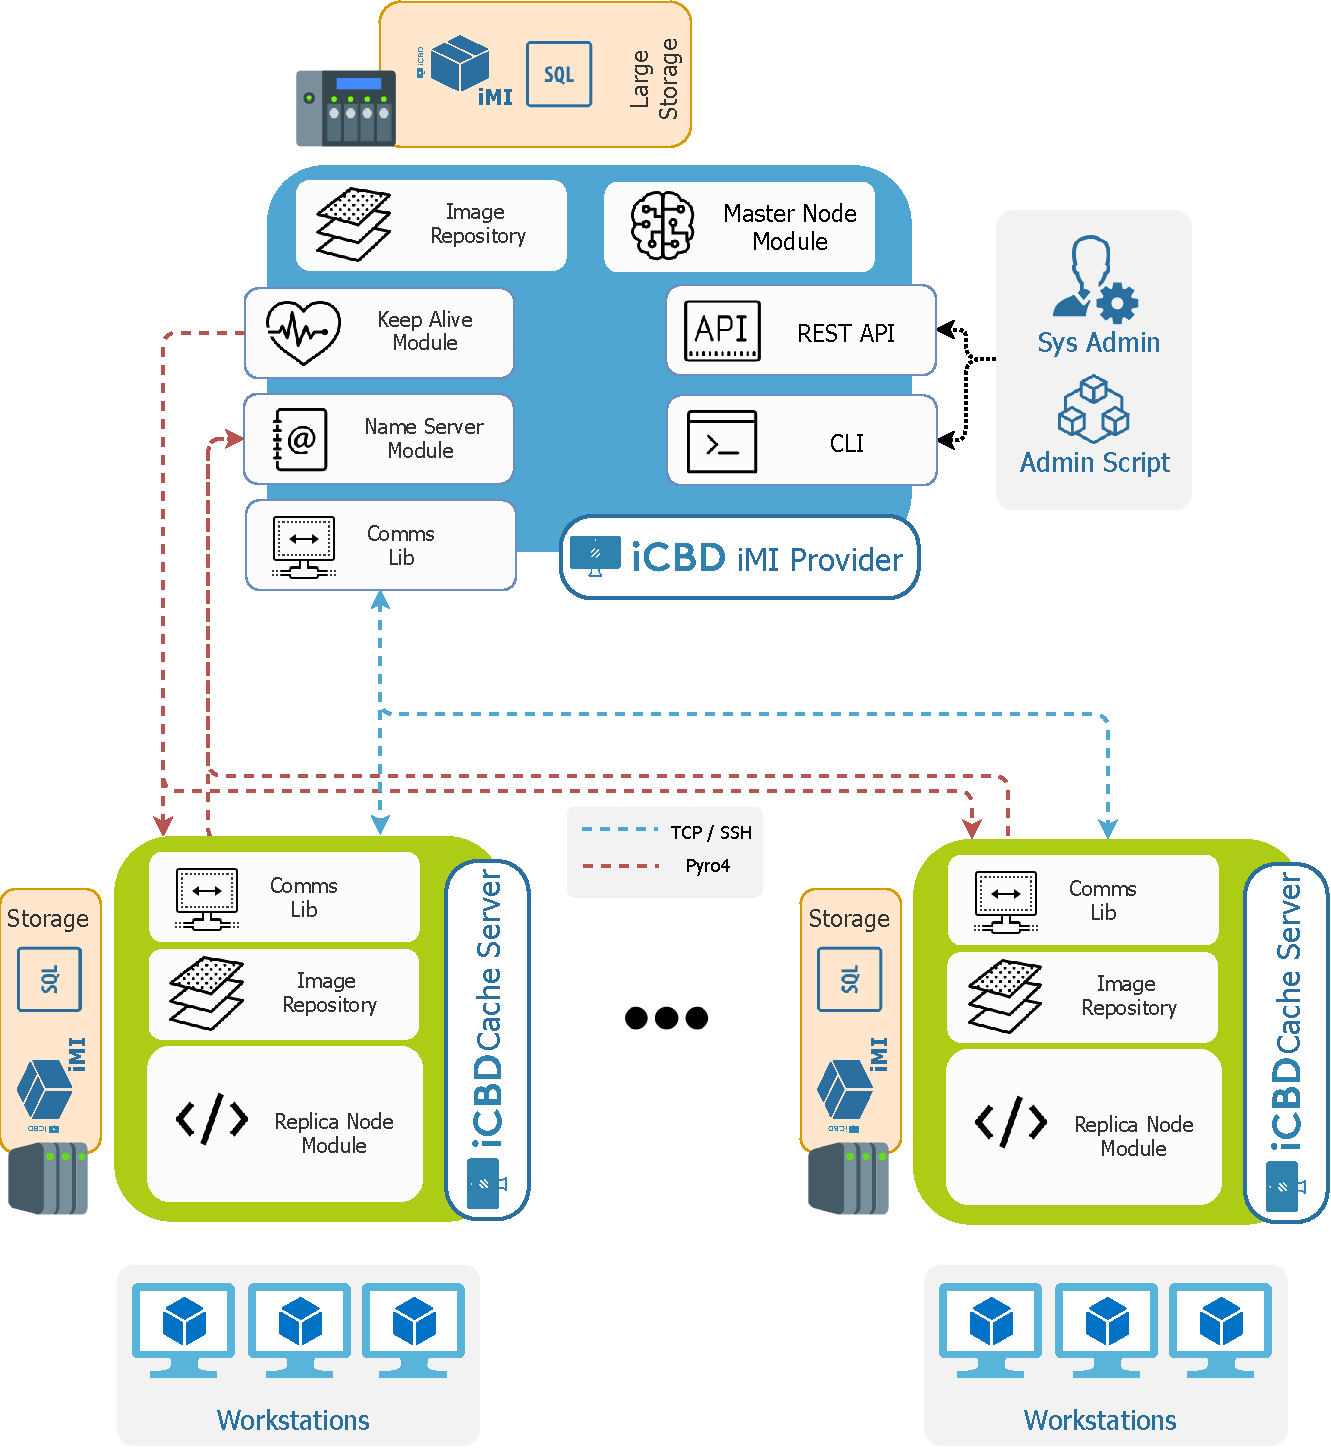
\includegraphics[height=4in, width=\textwidth]{cap4_icbd_arquit}
	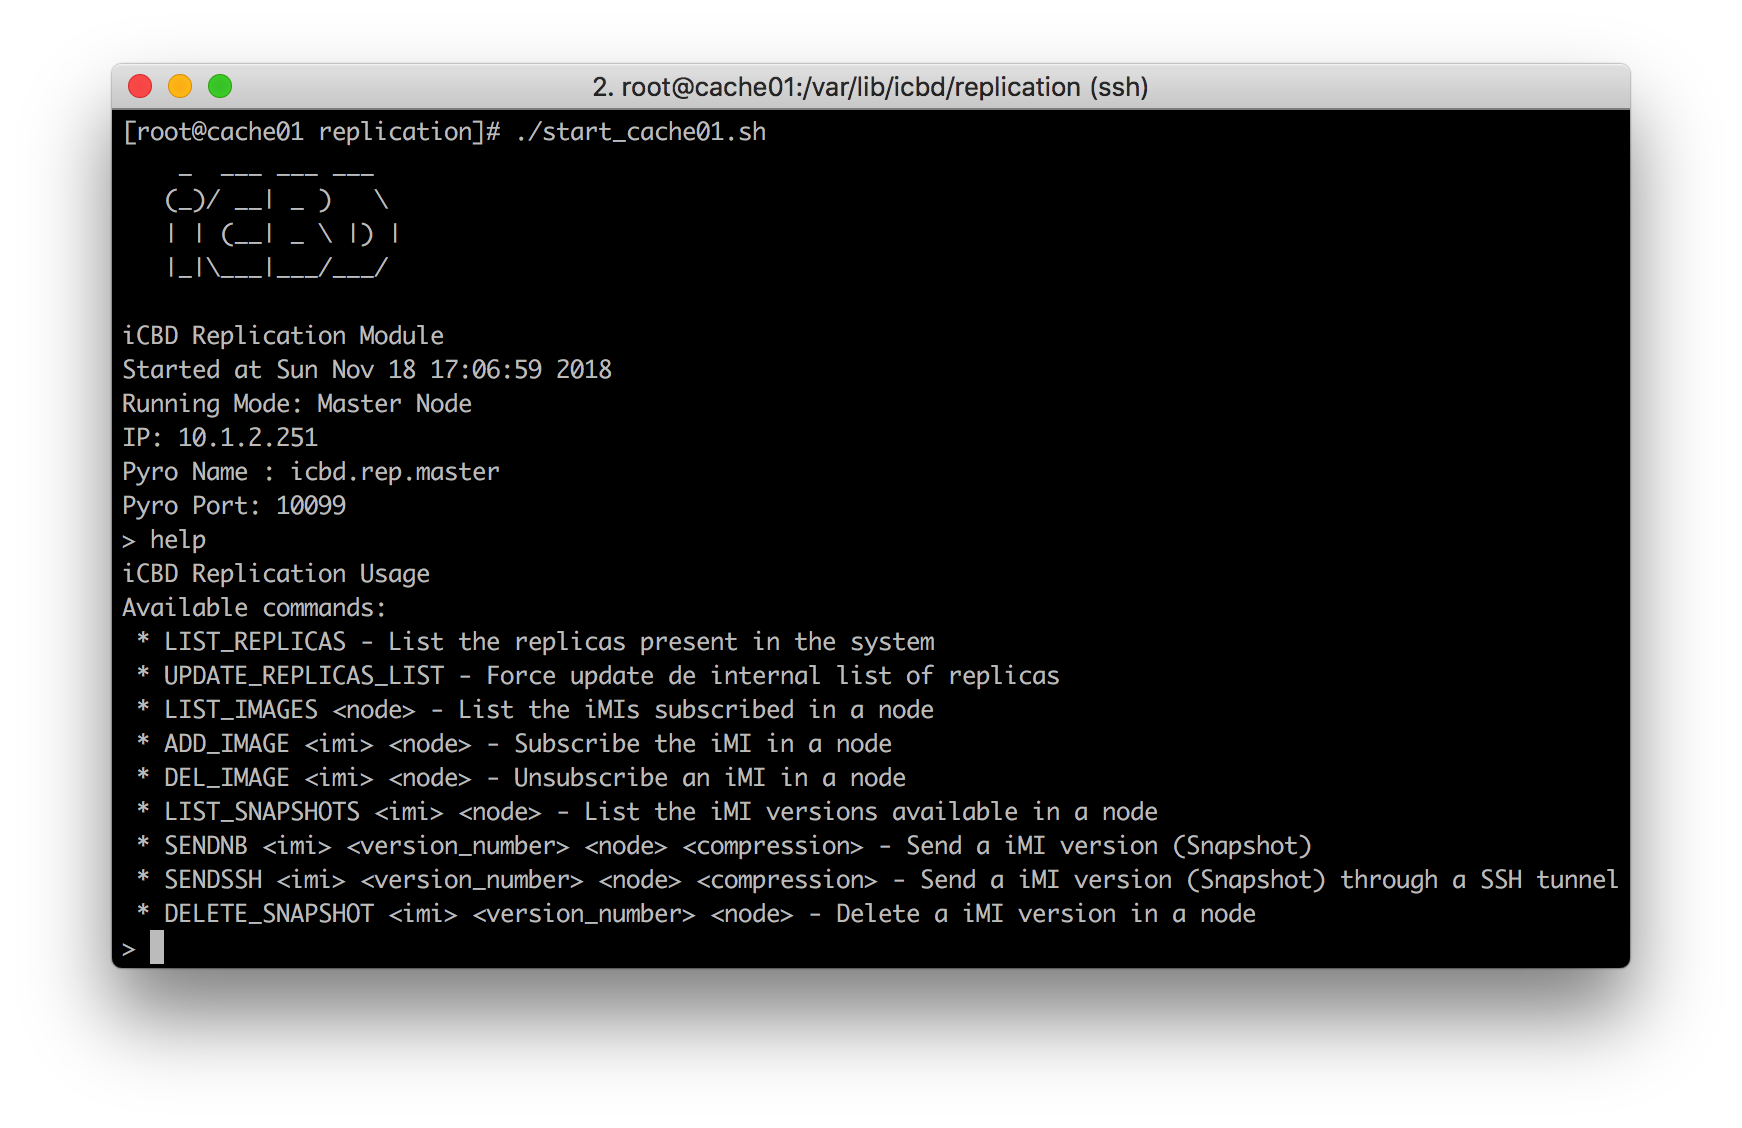
\includegraphics[width=\textwidth]{cap4_clihelp}
	\caption{iCBD Replication Module help output}
	\label{fig:icbd_rep_clihelp}
\end{figure}

%This interface, although simplistic, allows to efficiently manage all the tasks related to the replication of iMIs between the several servers of the platform. Following we demonstrate the functions provided by this interface and the effects produced on the platform:

Following we demonstrate the functions provided by this interface and the effects produced on the platform:

\begin{description}
	\item \texttt{List Replicas} - At any time it is possible to consult which nodes are registered in the platform, this command allows to list the replicas registered in the Name Server and indicates which URI is used to make a connection.
	%
	\item \texttt{Force Update Name Server} - As previously explained, when a replica node stops responding, that node is deleted from the records held by the Name Server. However, this process may not be immediate because of the timeout implemented. So this feature forces an update to the Name Server list by contacting all the nodes and determining if they are working correctly.
	%
	\item \texttt{List Subscribed iMIs} - This command receives as a parameter a replica node and shows a list of which iMIs that node is interested in receiving. It should be noted that a replica node may not subscribe to an iMI but still make it available to its client (was previously subscribed and the data was not deleted), it just will not be receiving new versions as they are being produced.
	%
	\item \texttt{Subscribe iMI} - Like the previous operation, this receives some arguments (a replica node and an iMI), then, registers the interest of the replica node in a given iMI. After this procedure, this node will be able to receive versions of this iMI.
	%
	\item \texttt{Unsubscribe iMI} - When a replica node ceases to be interested in a given image present on the platform, this operation marks that new versions of the iMI should not be transferred to that node. However, all versions that have already been sent persist on the node and in order to be deleted them an appropriated operation must be used.
	%
	\item \texttt{List iMI available versions} - It is usual for a given node to contain multiple versions of an iMI (for example, the Master Node contains all versions of all iMIs that can be distributed). Thus, given an iMI, this operation allows the listing of which versions a node stores.
	%
	\item \texttt{Send iMI Snapshot} - Possibly the most significant operation in this module. It is responsible for sending the respective versions of an iMI to the intended node. Always verifying which versions are present on the target node since only the differences between versions should be sent. This command also supports the application of a compression algorithm from those provided by the platform, since it may be the case of transferring a version for the first time with a very significant data volume, or the changes between versions possess a high compression rate thus making the compression of these data advantageous.
	%
	\item \texttt{Send iMI Snapshot Secure Connection (SSH)} - This functionality is similar to the one presented above. In particular case, they share a large portion of the code, because they carry out the same operations. They only differ in the method of sending the data, which in this instance are transmitted in an encrypted fashion through an SSH tunnel. This functionality is sure to add some overhead to the transfer process, but the encryption of the data is essential in situations where the nodes are in separate networks, where there is no control wheresoever to the data security.
	%
	\item \texttt{Delete iMI version} - Finally, it is necessary to provide a way to delete versions of a given IMI in a node. Either because no longer is desired to make an IMI available or for reasons of proper management the storage space on a replica node. It is important to note that because of the way different versions of iMIs are stored in the platform, deleting older versions may not result in a space release equal to the size of the full iMI, since newer versions probably will still need this data.
\end{description}


\subsubsection{REST API}
\label{subsub:impl_icbdrep_restapi}

In order to complement the Comand-Line Interface previously presented and creating a more straightforward, more ubiquitous way of interacting with the replication platform, a Rest API has been introduced. Aiming to provide the same functionalities as the CLI but trying to create the roots of a component that deals well with platform scaling and the introduction of new features or components.

In order to integrate this component with the remaining replication platform, we employ one of the most used frameworks for creating web platforms in Python, the Flask micro-framework.

\begin{listing}[ht]
\begin{description}
	\item \texttt{GET /api/replicas} - list all Replicas in the system
	\item \texttt{GET /api/replicas/\{replica\}/imis} - list of the iMis present in a Replica 
	\item \texttt{GET /api/replicas/\{replica\}/imis/subscribe/\{imi\}} - Replica subscribe to iMI 
	\item \texttt{GET /api/replicas/\{replica\}/imis/unsubscribe/\{imi\}} - Replica unsubscribe to iMI 
	\item \texttt{GET /api/replicas/\{replica\}/imis/\{imi\}/versions} - list the versions of iMI present in Replica
	\item \texttt{GET /api/replicas/\{replica\}/imis/\{imi\}/versions/\{version\}/delete} - delete a version of iMI in Replica
	\item \texttt{GET /api/master/imis/} - list the iMIs present in Master
	\item \texttt{GET /api/master/imis/\{imi\}/versions} - list versions of iMIs present in Master
	\item \texttt{GET /api/master/send?imi=\{imi\}\&version=\{version\}\&replica=\{replica\}} - send version of iMI to Replica
\end{description}
\caption{iCBD-Replication REST API Route Mapping}
\label{listing:impl_restapi}
\end{listing}

\paragraph{Flask}
\label{par:impl_flask}

Started as an April's Fool's Day joke to become the second most popular web development frameworks. Flask is a Python micro web framework designed with simplicity in mind, enabling quick deployment of applications and at the same time providing the ability to scale for complex environments. Such library enables the development of web applications without having to worry with more low-level aspects like network protocols and thread management. This framework began its development in 2010 by Armin Ronacher as a wrapper of two of his libraries: Werkzeug and Jinja.

Our use of this framework has focused only on its ability to quickly provide an environment for creating a REST API and connecting it with the rest of the replication platform. 
Next, we present the endpoints through which it is possible to interact with a master node:


%\begin{listing}[ht]
%\inputminted{python}{./Chapters/Code/cap4_restapi}
%\caption{iCBD-Replication REST API}
%\label{listing:impl_restapi}
%\end{listing}

%\textbf{TOPICS :}
%\begin{itemize}
%	\item Flask lib
%	\item Endpoints
%\end{itemize}


%%-------------------------------------------------------------------
%%	4. - Replica Node
%%-------------------------------------------------------------------
\subsection{Replica Node}
\label{sub:impl_icbdrep_replica_node}

The replica node introduces a lightweight module that is responsible for facilitating the process of transferring and updating the iMIs that are closest to the clients.
This module responds to the question of how to simplify the process of making available iMIs closer to the client. Complementing the remaining modules of the iCBD platform, here the focus is on implementing the logic of receiving snapshots, as well as providing a way to manage which iMIs are subscribed with their different versions. With these features, we have all the components to build a cache server, something that will be explained in detail in the section~\ref{sec:impl_cache_server}.

Contrasting with the Master Node, it is not possible to interact directly with a replica; all operations will always be conducted through a Master who then is in charge of communicating with the Replica, asking him to perform those actions. This fact is more than an architectural design choice, this way we meet one of the requirements that define that a cache server should be as light as possible leaving the platform management element to a centralised location not needing to know anything concerning the overall platform state. However, there are parts in common. Similarly to the Master Node one of the components present is an Image Repository, which in this case, manages locally the iMIs and respective versions.

\paragraph{Receiving a Snapshot}
\label{par:impl_receive_snap}
By far, this functionality is the reason for the existence of this module. The process of receiving a version of an iMI is complementary to the send process explained in Section~\ref{par:impl_sendsnap} even though much more straightforward. 
As explained, the \texttt{send()} operation needs some computation resources since it has to calculate all the differences between versions to transfer, and after that step create a stream of operations that when executed recreate precisely the differences between versions. 
So, on the receiving side of this stream (in this case the Replica Node), the \texttt{receive()} operation only is only required to receive the stream, decode the operations to administer to the file system and execute them.


%\textbf{TOPICS :}
%\begin{itemize}
%	\item Operations on the local repository
%	\item The receive operation
%\end{itemize}




%%-------------------------------------------------------------------
%%	4. - Building a iCBD Cache Server
%%-------------------------------------------------------------------
\section{Deploying an iCBD Platform with a Cache Server}
\label{sec:impl_cache_server}

%To solve some of the enunciated problems with a DaaS solution that derive from limited bandwidth, latency and jitter from the limitation of accessing the image repositories from an internet connection and provide some scalability feature with the implementation of proximity cache servers are key. These cache servers can store replicas of the iMIs created and maintained in an administration server. Moreover, since they are located in the same LAN segment as the clients is from here that they will boot.
%For accomplishing this work, the cache servers need to have hard drives. (Although it would be possible to have diskless cache servers, they would be blocked if there was an interruption in the internet access, and it is to avoid that the local drives are necessary. )

%A instalação, configuração e administração dos cache-servers far-se-á também pela instanciação a partir da imagem de uma VM especialmente preparada para o efeito e residente na cloud, no sistema de administração. Os cache-servers arrancam inicialmente pela rede a partir do servidor na cloud e carregam um Linux que vai formatar os discos, neles instalando o conteúdo da própria imagem de VM, terminando com a instalação de um boot loader que irá arrancar o sistema do cache-server após a máquina fazer reboot. Daí em diante o sistema de administração na cloud irá disponibilizar as actualizações que forem necessárias, podendo mesmo forçar a re-instalação total dos cache-servers.

%Note-se que uma vez instalado um cache-server numa LAN, dada a grande fiabilidade que pode ser ainda reforçada através das técnicas habituais em sistemas tolerantes a faltas e de elevada disponibilidade (referir a sugerida pelo Paulo), torna-se viável a utilização de servidores diskless, instanciados a partir de VMs templates configuradas e administradas na cloud e depois replicadas para o cache-server, como nas imagens dos desktops.

%Assim como o Linux dos cache-servers é instalado nos discos locais dos servidores a partir de imagens na cloud, é possível fazer o mesmo com qualquer outra imagem de Linux que se queira. Assim, o administrador de sistema de um cliente poderá configurar outras VMs com o software e os serviços de que necessitar, designar uma máquina física como alvo, e fazer com que a VM seja vertida para os discos da sua máquina física, sendo configurado um boot loader para lhe permitir arrancar com essa configuração.

%Como os clientes nestas categorias tipicamente necessitam de dezenas, centenas ou mais de postos de trabalho, na prática é impossível suportá-los directamente a partir de repositórios remotos de VMs templates. Em vez disso, iremos recorrer a “servidores de proximidade” ou “c​ache-servers”​, máquinas Linux reais ou virtuais devidamente dimensionadas e configuradas, instaladas na LAN dos clientes, idealmente uma (ou mais) por cada segmento de rede, as quais manterão réplicas das VMs templates a que cada cliente tem acesso nos repositórios remotos.
%Com estes cache-servers localmente acessíveis aumentar-se-á drasticamente a velocidade de transferência de dados e a latência e o jitter nos acessos reduzir-se-ão a valores insignificantes, podendo cada cache-server suportar dezenas (ou mais) de PCs clientes (estimamos o número em 15 a 30 por cada interface gigabit nos cache-servers, estimativa que permanece válido para PCs clientes ligados a 100 Mbps através de switches com ligação gigabit aos cache-servers).

Once the process of creating a mechanism to support the replication of iMIs has been completed, we have reached the stage where we tackle the problems of supporting a large number of clients, such a: limited bandwidth between a central repository and the workstations; high latency and jitter derived from network congestion or configuration errors in network equipment. So we believe that bringing the iMIs closer to the workstations is the way to solve all these problems.

At the beginning of this work, there already existed in the DI infrastructure an iCBD installation, but it was limited to only one Virtual Machine very limited regarding its resources and a couple of clients (also VMs), not to mention that the version of the platform as badly outdated and missing important features since implemented. Those limitations originated from the fact that the platform was sharing the same already scarce infrastructure as the remaining research projects and services of the department

All of this changed with the acquisition of new equipment for the exclusive use of this project, which became the perfect circumstance to think about the general architecture of the services and carry out a fresh installation of the whole platform.


\subsection{The infrastructure}
\label{sub:impl_infrastructure}

At our disposal is a modern infrastructure, including a two-node cluster - HPE ProLiant DL380 Gen9, interconnected by an HPE Flexfabric 5700 managed switch with 10Gbps links and storage provided by an HPE MSA 2040 SAN Storage Disk Array.
According to project requirements, the cache server should be supported by a low-cost machine, for this purpose, a desktop PC used in another research project was reconditioned, making it only a few modifications, such as, upgrading the amount of RAM and adding a second hard disk.
We can also count on using two teaching laboratories of the Department of Computer Science (Labs. 110 and 112) where each one contains 15 modern workstations (CPU - Intel Core i3-7100 @ 3.90GHz; RAM - 8 GB; Gigabit Lan) able to support virtualisation, to serve as clients of the platform.

The general specifications of all these components can be found in the tables~\ref{tab:imple_hp}, ~\ref{tab:imple_msa} and ~\ref{tab:imple_cs}.


\begin{table}[htpb]
\centering
\begin{tabular}{ll}
\textit{\textbf{CPU}}             & 2x Intel Xeon E5-2670 v3 @ 2.30GHz        \\
\textit{\textbf{Memory}}          & 128 GB                                    \\
\textit{\textbf{Controller Type}} & 12Gb/s SAS                                \\
\textit{\textbf{Ethernet}}        & 2 ports at 10 Gbps plus 4 ports at 1 Gbps \\
\textit{\textbf{Hypervisor}}      & VMware ESXi, 6.5.0, 4564106              
\end{tabular}
\caption{Specifications of one HP ProLiant DL380 Gen9 host}
\label{tab:imple_hp}
\end{table}

\newpage

\begin{table}[htpb]
\centering
\begin{tabular}{ll}
\textit{\textbf{Controllers}}    & 2 MSA 2040 SAS                          \\
\textit{\textbf{Total Capacity}} & 7.2 TB                                  \\
\textit{\textbf{Disks}}          & 12 HP SAS 600GB 10k Rpms                \\
\textit{\textbf{Host interface}} & 8 12Gb/sec SAS ports (4 per controller) \\
\textit{\textbf{Ethernet}}       & 2 ports at 1 Gbps (1 per controller)   
\end{tabular}
\caption{Specifications of the HPE MSA 2040 SAN Storage}
\label{tab:imple_msa}
\end{table}

\begin{table}[htpb]
\centering
\begin{tabular}{ll}
\textit{\textbf{CPU}} 		& Intel Core i5-650 @ 3.20GHz \\
\textit{\textbf{Memory}} 	& 12 GB \\
\textit{\textbf{Storage}} 	& 2x SATA 80 GB  + SATA 160 GB \\
\textit{\textbf{Ethernet}} 	& 2 ports at 1 Gbps \\
\textit{\textbf{OS}} 		& CentOS 7 3.10.0-514
\end{tabular}
\caption{Specifications of the Cache Server}
\label{tab:imple_cs}
\end{table}



\paragraph{Network}
\label{par:impl_infra_network}

Since it is intended that the iCBD platform coexist with other services and integrate into existing networks, we categorised the types of traffic that will be produced. We have internal traffic restricted to the platform - resulting from the execution of the various iCBD services and communication between them; and external traffic - which is an effect of accesses to the Internet or the act sending iMIs to workstations in the laboratories.

In the cluster, we have a virtualisation architecture based on the VMware solution, which makes available, as part of the VSphere suite, a centralised interface for virtual machine networking called Distributed Switch, from which one can configure, VM connections to switches for the entire cluster. 

\begin{description}
	\item [\textit{DI Distributed VSwitch}] - This switch holds five port groups, two corresponding to the networks of the laboratories, and the rest are networks used by various services of the department with differentiating levels of access (students, teachers, public).
	%
	\item [\textit{iCBD Distributed VSwitch}] - The networks present in this switch are only visible within the cluster, having as a role to differentiate the types of traffic produced: a management network; another for the administration of iMIs, and the remaining ones for traffic generated in tests of the platform and the Replication and Caching System.
\end{description}

Taking advantage of that two Distributed Switches were configured, each corresponding to one of the two traffic types listed above, in order to compartmentalise and not have platform traffic running through networks used daily by the department. Each PortGroup referenced in table~\ref{tab:impl_dvs} corresponds to a different network.

\begin{table}[]
\centering
\begin{tabular}{ll|ll}
\multicolumn{2}{c|}{\textbf{DI Distributed VSwitch}} & \multicolumn{2}{c}{\textbf{iCBD Distributed VSwitch}} \\ \hline
\multicolumn{1}{c}{\textit{Port Group}} & \multicolumn{1}{c|}{\textit{VLAN}} & \multicolumn{1}{c}{\textit{Port Group}} & \multicolumn{1}{c}{\textit{VLAN}} \\
DMZ-PRIV-DI & DMZ-PRIV-DI & iCBD-Adm-Net & VMWARE\_VMOTION\_DI \\
DMZ-PUB-DI & DMZ-PUB-DI & iCBD-Ceph & VMWARE\_VMOTION\_DI \\
LAB-DI-110 & LAB-DI-110 & iCBD-Net & VMWARE\_VMOTION\_DI \\
LAB-DI-112 & LAB-DI-112 & iCBD-Rep & VMWARE\_FT\_DI \\
R-ENSINO-PRIV-DI & R-ENSINO-PRIV-DI &  & 
\end{tabular}
\caption{Specifications of all Networks}
\label{tab:impl_dvs}
\end{table}

%\subsection{System Overview}
%\label{sub:system_overview}

%%-------------------------------------------------------------------
%%	4. - Services
%%-------------------------------------------------------------------
\subsection{Services}
\label{sub:impl_cache_services}

\paragraph{Roles in the Platform}
\label{par:impl_roles}

The several services needed to deploy the platform can be grouped by the following roles:

\begin{description}
	\item [\textit{iCBD-imgs}]
	\item [\textit{iCBD-rw}]
	\item [\textit{iCBD-home}]
	\item [\textit{iCBD-cache}]
\end{description}

\paragraph{Installing iCBD Core Services}
\label{par:impl_install_icbd_core}
%Found a Centos 7 kernel bug.
%https://bugs.centos.org/view.php?id=14228
%https://bugzilla.redhat.com/show_bug.cgi

\paragraph{BTRFS bug found in CentOS 7 Kernel}
\label{par:impl_centos_bug}

As a curiosity during the process of building the \textit{iCBDimgs} VM, we found in a bug in a core component of the \textit{coreutils} tool introduced in the kernel version \texttt{3.10.0-693.5.2} of CentOS 7. The \texttt{cp} command when used with option \texttt{--reflink=always} fails with the indication "failed to clone 'someFile': Operation not supported". This behaviour was reported to both CentOS and Red Hat and was eventually resolved. A more in-depth description of this process can be found in Annex~\ref{ann:bug}.







